\section{Evaluation}


\begin{figure*}[tb]
    \centering
    \begin{subfigure}[b]{0.33\textwidth}
        \includegraphics[width=2.2in]{graph/wc_docker.eps}
        \caption{Exim - 120core}
    \end{subfigure}%
    \begin{subfigure}[b]{0.33\textwidth}
        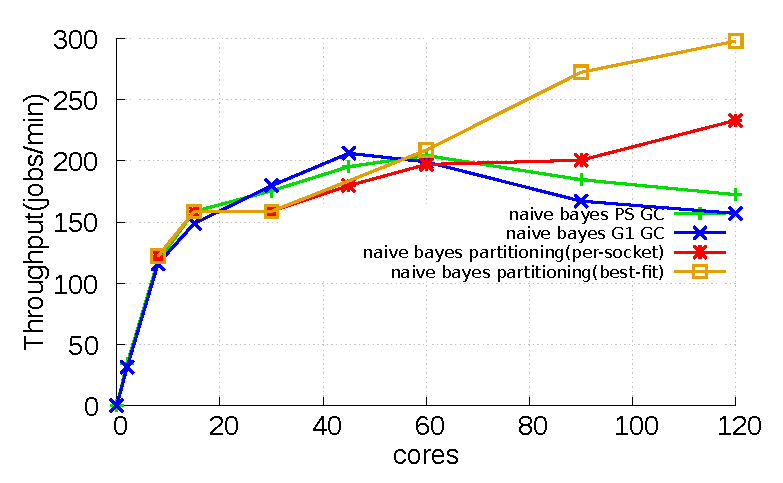
\includegraphics[width=2.2in]{graph/nb_docker.eps}
        \caption{Lmbench - 120core}
    \end{subfigure}%
    \begin{subfigure}[b]{0.33\textwidth}
        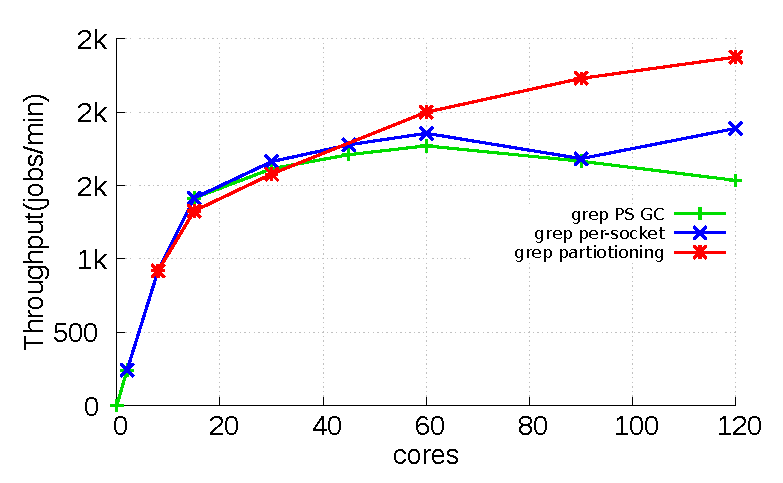
\includegraphics[width=2.2in]{graph/grep_docker.eps}
        \caption{AIM7 - 120core}
    \end{subfigure}
        \begin{subfigure}[b]{0.33\textwidth}
        \includegraphics[width=2.2in]{graph/pagerank_docker.eps}
        \caption{Lmbench - 120core}
    \end{subfigure}%
        \begin{subfigure}[b]{0.33\textwidth}
        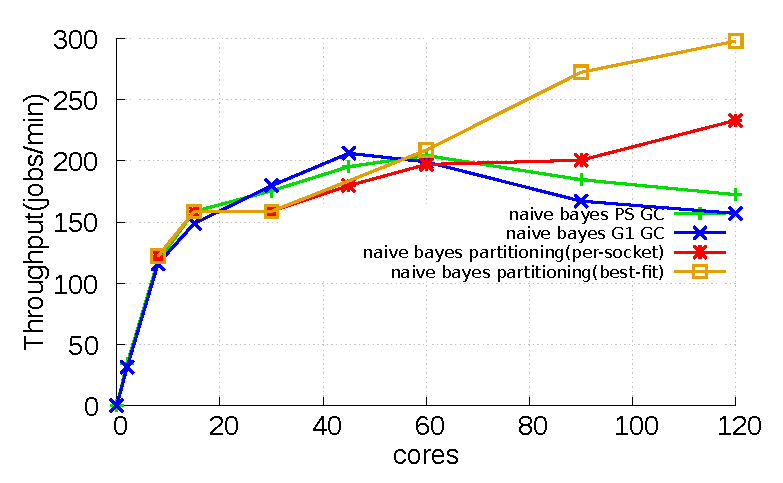
\includegraphics[width=2.2in]{graph/nb_docker.eps}
        \caption{Lmbench - 120core}
    \end{subfigure}%
        \centering
    \caption{CPU utilization on 120 core.}
    \label{fig:utilization3}
\end{figure*}





\begin{figure*}[tb]
    \centering
    \begin{subfigure}[b]{0.20\textwidth}
        \includegraphics[width=1.4in]{graph/wc_cpuutils.eps}
        \caption{Word Count}
    \end{subfigure}%
    \begin{subfigure}[b]{0.20\textwidth}
        \includegraphics[width=1.4in]{graph/wc_cpuutils.eps}
        \caption{Naive Basian}
    \end{subfigure}%
    \begin{subfigure}[b]{0.20\textwidth}
        \includegraphics[width=1.4in]{graph/wc_cpuutils.eps}
        \caption{Grep}
    \end{subfigure}%
        \begin{subfigure}[b]{0.20\textwidth}
        \includegraphics[width=1.4in]{graph/wc_cpuutils.eps}
        \caption{Pagerank}
    \end{subfigure}%
        \begin{subfigure}[b]{0.20\textwidth}
        \includegraphics[width=1.4in]{graph/wc_cpuutils.eps}
        \caption{Pagerank}
    \end{subfigure}
        \centering
    \caption{CPU utilization on 120 core.}
    \label{fig:utilization2}
\end{figure*}


%$$$$$$$$$$$$$$$$$$$$$$$$$$$$$$$$$$$$$$$$$$$$$$$$$$$$$$$$$$$$$$$$$$$$$$$$$$$$$$$$
%Paragraph 1: 실험 환경 설명
%$$$$$$$$$$$$$$$$$$$$$$$$$$$$$$$$$$$$$$$$$$$$$$$$$$$$$$$$$$$$$$$$$$$$$$$$$$$$$$$$
\ifkor
이번 장에서는 스파크의 Scalalbility에 대해서 설명한다. 실험 환경은 2장에서 수행한 방법과
같은 플랫폼에서 실험을 하였고, 

To evaluate the performance of we use well-known
three benchmarks:AIM7 Linux scalability benchmark, Exim email server in
MOSBENCH and lmbench.
We selected these three benchmarks because they are fork-intensive workloads and
exhibit high reverse mapping lock contentions.
Moreover, AIM7 benchmark has widely been used in practical area not only for testing the
Linux but also for improving the scalability. 
To evaluate deferu for real world
applications, we use Exim which is the most popular email server.
A micro benchmark, Lmbench, has been selected to focus on Linux fork operation-intensive
fine grained evaluations.
%Finally, we wanted to focus on Linux fork performance and scalability;therefore,
%we selected lmbench, a micro benchmark.

%Paragraph 3: 운영체제 및 커널 버전 설명
We ran the three benchmarks on Linux 3.19.rc4 with stock Linux with 
the automatic NUMA balancing feature disabled because the
Harris linked list has the iteration issue~\cite{petrank2013lock}. 
All experiments were performed on a 120 core machine with 8-socket, 15-core
Intel E7-8870 chips equipped with 792 GB DDR3 DRAM.
\else

\fi




%$$$$$$$$$$$$$$$$$$$$$$$$$$$$$$$$$$$$$$$$$$$$$$$$$$$$$$$$$$$$$$$$$$$$$$$$$$$$$$$$
%Paragraph 2: 비교 대상 설명
%$$$$$$$$$$$$$$$$$$$$$$$$$$$$$$$$$$$$$$$$$$$$$$$$$$$$$$$$$$$$$$$$$$$$$$$$$$$$$$$$
\ifkor
이번 장에서는 스파크의 Scalalbility에 대해서 설명한다. 첫째로 
둘째로, NUMA socket 단위로 파티션닝을 수행한 방법이다. 우리의 시스템은 한 소켓당 15코어를
가지는 NUMA machine이므로 15개의 코어를 가지는 도커를 8개를 생성하여 동작시켰다.
다음으로, system의 영향을 가장 덜받을 수 있는 코어인 8,7개 단위로 하여 실험하였고, 
마지막으로 더 적은 코어로 파티션하는것에 대한 효과를 보기 위해 4개의 코어 단위로 나누어 측정하였다. 
\else

\fi




%$$$$$$$$$$$$$$$$$$$$$$$$$$$$$$$$$$$$$$$$$$$$$$$$$$$$$$$$$$$$$$$$$$$$$$$$$$$$$$$$
%Paragraph 2: A그룹에 대한 실험 결
%$$$$$$$$$$$$$$$$$$$$$$$$$$$$$$$$$$$$$$$$$$$$$$$$$$$$$$$$$$$$$$$$$$$$$$$$$$$$$$$$
\ifkor
실험 결과 먼저 소켓단위로 파티션한 것은 
이번 장에서는 스파크의 Scalalbility에 대해서 설명한다.
%Paragraph 1: 워크로드에 대한 설명
AIM7 forks many processes, each of which concurrently runs. 
We used AIM7-multiuser, which is one of workload in AIM7.
The multiuser workload is composed of various workloads such as disk-file
operations, process creation, virtual memory operations, pipe I/O, and
arithmetic operation.
To minimize IO bottlenecks, the workload was executed with tmpfs filesystems, each
of which is 10 GB.
To increase the number of users during our experiment and show the results at the
peak user numbers, 
we used the crossover.

%Paragraph 2: 실험 결과에 대한 설명
The results for AIM7-multiuser are shown in Figure~\ref{fig:aim7}, and the
results show the throughput of AIM7-multiuser with four different settings.
Up to 60 core, the stock Linux scales linearly while serialized updates in
Linux kernel become bottlenecks. 
However, up to 120core, unordered harris list and our \deferu scale well because
these workloads can run concurrently updates and can reduce the locking
overheads due to reader-writer semaphores(\code{anon\_vma},
\code{file}).
The combination of deferu with unordered harris list has best performance and
scalability outperforming stock Linux by 1.7x and unordered harris list by
1.1x.
While the unordered harris list has 19\% idle time(see
Table~\ref{tab:memuse}), stock Linux has 51\% idle time waiting to acquire
both \code{anon\_vma's rwsem} and \code{file's i\_mmap\_rwsem}.
We can notice that although deferu has 23\% idle time, the throughput is higher than
unordered harris list.
In this benchmark, the ordered harris list has the lowest performance and
scalability because their \code{CAS} fails frequently.

%Paragraph 2: 실험 결과에 대한 설명
The results for AIM7-multiuser are shown in Figure~\ref{fig:aim7}, and the
results show the throughput of AIM7-multiuser with four different settings.
Up to 60 core, the stock Linux scales linearly while serialized updates in
Linux kernel become bottlenecks. 
However, up to 120core, unordered harris list and our \deferu scale well because
these workloads can run concurrently updates and can reduce the locking
overheads due to reader-writer semaphores(\code{anon\_vma},
\code{file}).
The combination of deferu with unordered harris list has best performance and
scalability outperforming stock Linux by 1.7x and unordered harris list by
1.1x.
While the unordered harris list has 19\% idle time(see
Table~\ref{tab:memuse}), stock Linux has 51\% idle time waiting to acquire
both \code{anon\_vma's rwsem} and \code{file's i\_mmap\_rwsem}.
We can notice that although deferu has 23\% idle time, the throughput is higher than
unordered harris list.
In this benchmark, the ordered harris list has the lowest performance and
scalability because their \code{CAS} fails frequently.
\else

\fi




%$$$$$$$$$$$$$$$$$$$$$$$$$$$$$$$$$$$$$$$$$$$$$$$$$$$$$$$$$$$$$$$$$$$$$$$$$$$$$$$$
%Paragraph 2: b,c 그룹에 대한 실험 결
%$$$$$$$$$$$$$$$$$$$$$$$$$$$$$$$$$$$$$$$$$$$$$$$$$$$$$$$$$$$$$$$$$$$$$$$$$$$$$$$$
\ifkor
이번 장에서는 스파크의 Scalalbility에 대해서 설명한다.
\else

\fi



%$$$$$$$$$$$$$$$$$$$$$$$$$$$$$$$$$$$$$$$$$$$$$$$$$$$$$$$$$$$$$$$$$$$$$$$$$$$$$$$$
%Paragraph 2: CPU utilization에 대한 설명
%$$$$$$$$$$$$$$$$$$$$$$$$$$$$$$$$$$$$$$$$$$$$$$$$$$$$$$$$$$$$$$$$$$$$$$$$$$$$$$$$
\ifkor
이번 장에서는 스파크의 Scalalbility에 대해서 설명한다.
\else

\fi
